\section{Durchführung}
\subsection{Aufbau}
Ein Blockschaltbild des in diesem Versuch verwendeten Blockschaltbilds ist in \autoref{fig:block}
dargestellt.
\begin{figure}
    \centering
    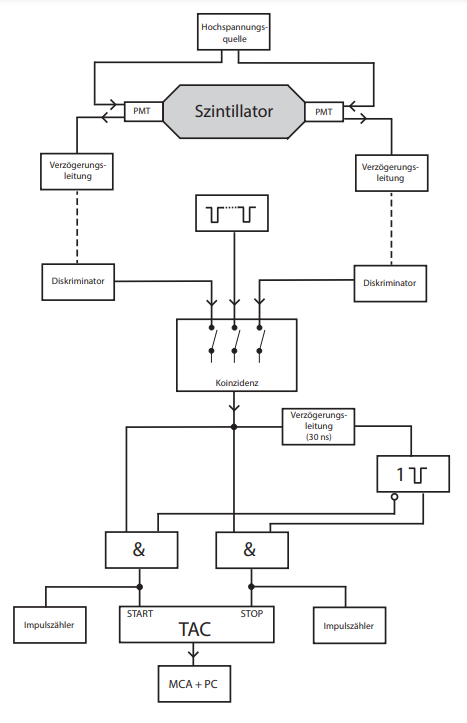
\includegraphics[width=0.67\textwidth]{block.png}
    \caption{Blockschaltbild des Versuchaufbaus \cite{anleitung}.}
    \label{fig:block}
\end{figure}
In diesem Versuch werden die Myonen mit einem $50 \;$l Szintilatortank detektiert. Das Szintilatormaterial 
ist hier organisch, was den Vorteil einer geringeren Abklingzeit aber den Nachteil einer schlechteren Energieauflösung 
gegenüber anorganischen Detektoren hat. Das hier verwendete Material hat eine Abklingzeit von $10$\;ns.\\
Der Szintilatortank ist an beiden Seiten an Photomultiplier angeschlossen. Photomultiplier wandeln die Lichtimpulse 
des Szintilators in eletrische Impulse um.
Um falsche Impulse und elektronisches Rauschen zu unterdrücken sind beide Photomultiplier über eine 
Koinzidenzschaltung gekoppelt welche nur Signale zulässt wenn beide Photomultiplier gleichzeitig Impulse 
ausgeben. Da die Photomultiplier bauliche Unterschiede aufweisen können sind beiden Verzögerungsleitungen 
nachgeschaltet damit gleichzeitige Signale auch gleichzeitig in der Koinzidenz ankommen.
Vor der Koinzidenz sind außerdem jeweils Diskriminatoren verbaut, welche der Rauschunterdrückung dient. 
Alle Signale unterhalb einer einstellbaren Schwelle werden dabei herausgefiltert. 
Des Weiteren dienen sie dazu, die eingehenden Signale auf eine einheitliche Länge und Breitere zu normieren.\\
Der Koinzidenz folgend ist eine logische Schaltung und ein TAC (Zeit-Amplitude-Konverter). Letzterer misst die 
Zeit zwischen einem eingehenden Start und einem Stopsignal und gibt eine Amplitude proportional 
zu dieser auf einen Vielkanalanalysator und dann an ein Auswertungsprogramm auf einem Computer.
Die Zahl der Start- und Stopsignale wird außerdem durch weitere Impulszähler gemessen. \\
Die meisten Myonen durchqueren den Szintilator ohne zu zerfallen und lösen damit am TAC nur ein Startsignal, 
aber kein Stopsignal aus. Eine logische Schaltung aus zwei AND-Gattern und einer monostabilen Kippstufe wird dem TAC 
also vorgeschaltet. Letztere setzt die Schaltung nach einer Suchzeit $T_{\text{S}}$ wieder in ihren 
Ausgangszustand zurück, sodass das nächste Signal wieder als Startsignal gewertet wird.
Der monostabilen Kippstufe ist außerdem eine Verzögerungsleitung von $30\;$ns vorgeschaltet.
Wenn anfangs ein Signal auf die Schaltung trifft, liegt eine Spannung am invertierten Ausgang der monostabilen Kippstufe an,
sodass das linke AND-Gatter in \autoref{fig:block} passiert werden kann und ein Startsignal ausgelöst wird. Das verzögerte Signal löst 
die Kippstufe aus, sodass im rechten AND-Gatter ein Signal passieren kann und somit ein Stopsignal aufgenommen werden kann.
Nach Eintreffen des Stopsignals oder nach Ablauf der Suchzeit löst die monostabile Kippstufe wieder aus und 
es kann das nächste Startsignal aufgenommen werden. \\
Trotz des Herausfilterns vieler Störeffekte kann es zu Fehlsignalen kommen, wenn zwei Myonen hintereinander 
den Szintilator auslösen. Das zweite Myon würde dabei als Stopsignal regristriert werden. Experimentell kann 
dieses Signal nicht von einem echten Signal unterschieden werden und muss in der Auswertung berücksichtigt werden.

\subsection{Justage und Durchführung}
Der oben beschriebene Aufbau wird schrittweise aufgebaut. 
Zunächst wird die Funktionalität der Photomultiplier mittels eines Oszilloskopes überprüft.
Wenn Impulse unterschiedlicher Höhen gemessen werden, werden in einem nächsten Schritt die Diskriminatoren 
so eingestellt, dass ca. 30 Impulse pro Sekunde gemessen werden können. Die Impulse sollten gleiche Höhe 
und Breite haben. Auch dies wird mit einem Oszilloskop überprüft und gegebenenfalls nachjustiert.
Anschließend werden Verzögerungsleitungen und die Koinzidenz angeschlossen. Die Koinzidenz wird auf einen Impulszähler 
gegeben. Die Zählrate wird in Abhängigkeit der eingestellten Verzögerung gemessen.
Für den Versuch wird dann eine geeignete Verzögerung gewählt an welcher die Zählrate maximal ist.
Anschließend muss der Vielkanalanalysator kalibriert werden. Dazu wird die gesamte Schaltung aufgebaut und 
mit einem Doppelimpulsgenerator Signale verschiedener Zeitdifferenzen auf die Schaltung gegeben und den ausgebenen
Kanälen zugeordnet und notiert.
Nach vollständigem Aufbau werden Messprogramm und Impulszähler gestartet.



